\documentclass{ucetd}
\usepackage{subfigure,epsfig,amsfonts}
\usepackage{natbib}
\usepackage{amsmath}
\usepackage{amssymb}
\usepackage{amsthm}
\graphicspath{ {figures/ch4/} }
\begin{document}
\chapter{Discussion}















\section{Summary}
%State of the field
Pulsed contractility is an increasingly common form of actomyosin contractility that is thought to play an important role in driving cell shape changes and tissue morphogenesis during development \cite{Gorfinkiel:2016bv}.  Pulsed contractions have been well characterized in \textit{Drosophila} tissues where they drive apical constriction of epithelial cells \cite{Rauzi:2011bk}.  On a subcellular level, pulsed contractions are characterized by cycles of local actomyosin assembly, contraction-mediated shape changes, and disassembly.  However, the mechanisms governing the initiation, termination, and spatial organization of pulsed contractions remain unclear.  One current model, known as the contractile instability model, postulates that pulsed contractions are initiated when local myosin II activity is self-amplified by the contraction-mediated accumulation of F-actin, Myosin II, and/or their upstream regulators (Figure 1.4) \cite{Bois:2011kx, Kumar:2014ux}.  Pulsed contractions terminate when either: i) Myosin II contractility promotes local network disassembly or ii.) tension built up within the network resists further deformation.  An alternate clustering model argues that pulsed contractions are initiated by mutual binding interactions between factors such Anillin and F-actin organize the cortex into patches has also been proposed \cite{Maddox:2005gd}.  A variant of this clustering model might involve Anillin positively feeding back onto RhoA directly, or indirectly through interactions with the GEF ECT-2 \cite{Piekny:2008jf, Frenette:2012do}. 

%My results
Here, we have definitively ruled out the contractile instability and clustering models as major mechanisms for initiating pulsed contractions in \textit{C.elegans}.  Instead, we propose a model in which local cycles of autocatalytic RhoA activation and delayed inhibition set the timing of actomyosin assembly, contraction, and disassembly within pulsed contractions.  We have shown that active RhoA begins to accumulate within pulsed contractions before downstream factors such as F-actin, Myosin II, and Anillin (Figure 2.4).  Our measurements reveal that active RhoA reaches a peak, and then begins to dissipate, before these factor as well (Figure 2.4).  Inconsistent with the contractile instability or clustering models, RhoA continues to pulse in the absence of Myosin II or Anillin (Figure 2.5, Figure 3.4).  We have established that the localization and dynamics of the Rho GAPs RGA-3/4 is consistent with their role in providing delayed negative feedback onto RhoA: GFP::RGA-3 accumulates with a delay relative to active RhoA and the deletion of RGA-3 and RGA-4 eliminates RhoA pulses (Figure 2.7).  Furthermore, we have established a potential mechanism for delayed inhibition of RhoA through F-actin-mediated recruitment of RGA-3/4 to the cortex.


%Figure 4.1
\begin{figure}[!htbp]
\centering
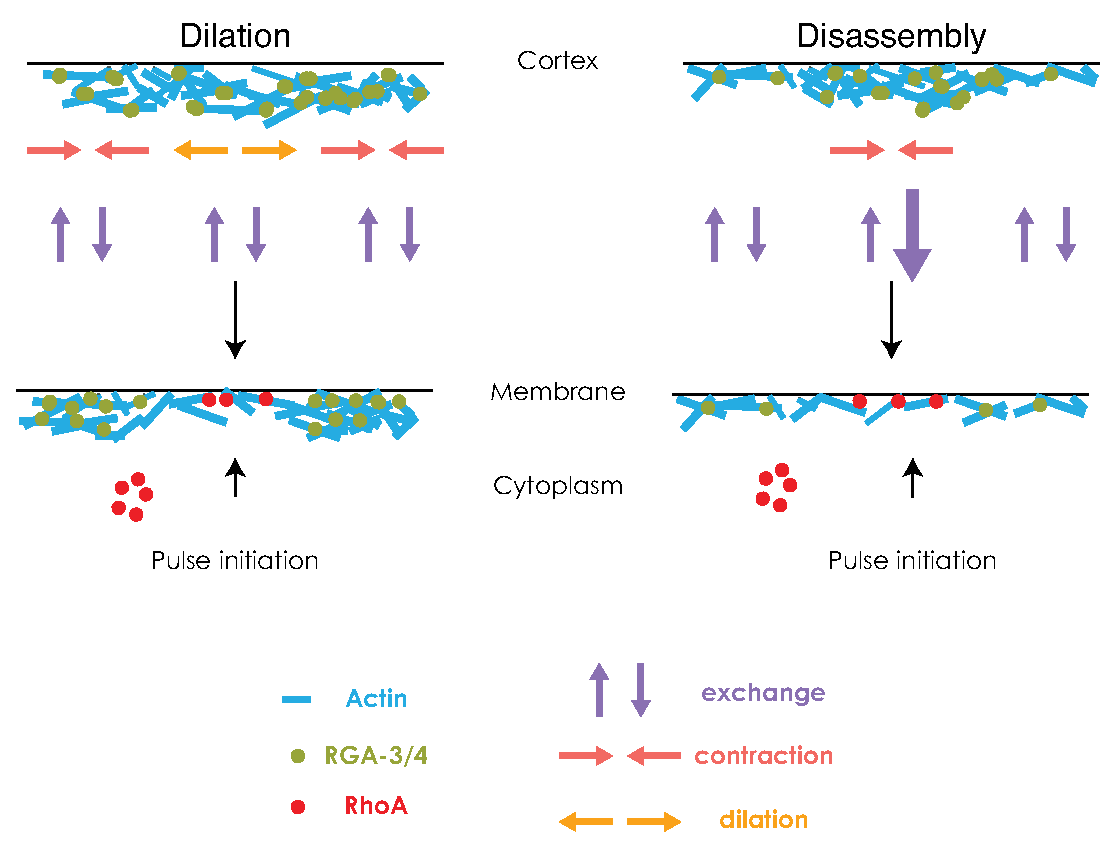
\includegraphics[width=\textwidth]{Figure4-1}
\captionof{figure}[Schematic of our novel conceptual model.]{\textbf{Schematic of our novel conceptual model.} Local pulses of active RhoA (red circles) can be triggered by a dilation (orange arrows) in the cortex (left) or local disassembly of actin filaments (cyan rods) (right).  Both dilation and disassembly lead to a decrease in F-actin, which in turn decreases RGA-3/4 (green circle) localization on the cortex.  In this model, local actin disassembly driven by myosin-mediated contractility (pink arrows).}
\end{figure}

\section{Proposed mechanism} 
Together, our results provide the basis for a novel mechanism for explaining pulsed contractions in particular, and cell shape changes in general.  In our current model, pulsed contractions are driven by autocatalytic activation of RhoA and terminated by the delayed recruitment of RGA-3/4 (Figure 2.9).  It is likely that we can rule out classic activator-inhibitor models in which pattern formation relies on long-range inhibition by a rapidly diffusing inhibitor \cite{Gierer:1972vq}.  Indeed, we have made two key observations.  First, the fact that GFP::RGA-3 strongly co-localizes with F-actin suggests that RGA-3 does not diffuse rapidly within the membrane (Figure 2.8).  Second, the depolymerization of F-actin leads to a rapid loss of GFP::RGA-3 on the cortex, and global activation of RhoA on the membrane (Figure 2.8).  We can therefore extend our model by considering how coupling RGA-3/4 activity to F-actin polymerization might spatiotemporally regulate RhoA activation and pulsed contraction dynamics.  Thus, a new model should contain the essential ingredients for an excitable system that exhibits spatial dynamics: the activator (RhoA) is autocatalytic, the inhibitor (RGA-3/4) provides delayed negative feedback, and the localization of inhibitor everywhere on the cortex ensures long-range inhibition.  Therefore, in order for RhoA to pulse on and off the cortex, stochastic fluctuations in active RhoA must exceed a threshold, or RGA-3/4 levels must locally decrease.  


%Local depletion of RGA-3/4
In principle, local RGA-3/4 levels could be modulated by dynamic changes of the underlying actin cytoskeleton.  In one scenario, local F-actin disassembly could lead to a decrease in RGA-3/4 levels, which could then promote the local accumulation of active RhoA (Figure 4.1).  We have often observed oscillations of pulsed contractions in AB embryos.  This observation is consistent with what our new model would predict: cycles of RhoA pulses are initiated by contraction-driven actin disassembly from the previous pulsed contraction.  Indeed, our single molecule measurements indicate that pulsed contractions are characterized by an increase in actin assembly during the initiation phase, and an increase in actin disassembly during the termination phase (Figure 2.3C,D).  In another scenario, large variations in contractility could drive tearing/dilations in the cortex (Figure 4.1).  A RhoA pulse would then form in the region that has been recently depleted of actin filaments.  Our preliminary observations suggests that multiple contracting pulses in close proximity could build up enough tension within the network to rupture nearby actin filaments, and promote the formation of a new pulsed contractions (Figure 4.2).  

%Figure 4.2
\begin{figure}[!htbp]
\centering
\includegraphics[width=0.85\textwidth]{Figure4-2}
\captionof{figure}[Myosin II pulses form in cortical regions depleted of RGA-3/4.]{\textbf{Myosin II pulses form in cortical regions depleted of RGA-3/4.} Micrograph of 1-cell stage embryo expressing GFP::RGA-3 and NMY-2::mKate.  The yellow arrowhead identifies a new pulsed contraction forming between two existing pulses.}
\end{figure}


%Model predictions
Although this model is currently speculative, it could in principle recapitulate all of our preliminary and well-established observations.  For example, this model would predict that global depletion of F-actin (or RGA-3/4) would lead to global activation of RhoA (Figure 2.7 and Figure 3.3).  This model would also predict that pulsed contractions are often preceded by local dilations in the cortex.  Indeed, our single molecule measurements indicate that the initiation of pulses often correlates with a dilation of the cortex (Figure 2.3G).  Furthermore, we would expect that perturbations that decrease the polymerization rate, or stability, of actin filaments to promote larger tears in the cortex pulses, and hence larger pulses.  Consistent with this prediction, we have observed larger pulses in \textit{cyk-1} (and \textit{pfn-1}) RNAi embryos in which local cortical dynamics are exaggerated relative to wild-type embryos (Figure 3.4, Figure 3.5).  Similarly, we would expect that perturbations that stabilize the actin cortex should either decrease the amplitude or duration of pulses, or eliminate them altogether.  For example, our observations suggest that RhoA pulses in \textit{nmy-2} RNAi embryos are not as robust as wild-type pulses, and they appear to terminate more rapidly.  Consistent with this result, we have observed that stabilizing actin filaments with the drug jasplakinolide also dampens active RhoA pulses (data not shown).  Thus, our new model provides a novel conceptual framework that has the capacity to explain our previous experimental results, as well as guide future experiments.



\section{Open Questions}
%How do you get different RhoA pulse dynamics
Although we have gained key insights into the mechanisms regulating pulsed contractility, many details of pulsed contractions are still not well understood.  For example, we currently understand very little about how pulsed contractions are regulated spatially.  What determines the size of a pulse?  Where is a pulsed contraction most likely to form on the cortex?  To what extent are neighboring pulses coupled?  What regulates the overall spatial pattern of pulsed contractions on the cortex?  Answering these questions might help to uncover, for example, why pulsed contractions in P0 embryos are different than pulsed contractions in AB embryos.  The cortex of P0 embryos is highly stereotyped, where pulses maintain a characteristic size and spacing throughout polarity establishment \cite{Munro:2004jk}.  In contrast, the size, number, and pattern of pulses in AB is much more variable.  In some AB embryos, pulsed contractions may oscillate in one region of the cortex for multiple cycles.  In other AB embryos, pulsed contractions that appear to be organized randomly on the cortex will be highly synchronized temporally, where each pulse initiates and terminates simultaneously.  Is RhoA locally activated in multiple cortical regions simultaneously?  Or, is RhoA globally activated?  How, then, would RhoA effectors spatially segregate into different pulses instead of forming one large pulse?  Other key differences between P0 and AB pulses are their duration and the extent to which they contract.  P0 pulses tend to be longer in duration and form deeper membrane invaginations than AB pulses.  This is surprising, as the initial kinetics of active RhoA accumulation is similar for P0 and AB pulses (Figure 3.5).  One possibility is that one or more factors downstream of active RhoA function differentially in P0 and AB.  For example, although Anillin is recruited to pulsed contractions in both AB and P0, we do not know to what extent Anillin is active in both contexts.  Depleting anillin causes P0 pulses to become shorter and contract less, resembling AB pulses (Figure 3.4,3.5).  Therefore, understanding how pulses in P0 differ from pulses in AB might provide clues to how different tissues in different organisms tune pulsed contractility to accomplish different tasks. 


%What limits the spread of local RhoA activation during a pulsed contraction
What limits the spread of local RhoA activation during a pulsed contraction?  Why do pulses of active RhoA not form traveling waves as they spread across the cortex?  One possibility is that RGA-3/4 laterally inhibits RhoA activation.  The presence of RGA-3/4 on actin filaments in close proximity to a pulsed contraction might inhibit active RhoA and prevent active RhoA from diffusing into nearby cortical regions and forming traveling waves.  This is consistent with our observation that pulses of RhoA activity spread in \textit{cyk-1} RNAi embryos, which presumably contain less RGA-3/4 on the cortex than wild-type embryos (see Chapter 3).  Another possible mechanism that prevents the spread of active RhoA might be the rapid depletion of a RhoA substrate.  However, this mechanism seems unlikely as the cortex of \textit{rga-3/4} RNAi embryos is hypercontractile and exhibits regular spacing between pulsed contractions (data not shown).  One promising possibility is that mutual binding interactions between RhoA and its effectors might prevent the diffusion of active RhoA out of pulsed contractions.  For example, we have shown that depletion of Rho kinase or Anillin causes RhoA activation to spread (see Chapter 3).  By simultaneously binding active RhoA, F-actin, septins, and/or Myosin II, Anillin could spatially restrict RhoA activation.  Understanding how active RhoA is spatially restricted to pulsed contractions might provide some insight, for example, into understanding how   


%What is the nature of positive feedback	that initiates RhoA pulses?
Our experiments in \textit{C.elegans}, as well as recent experiments in \textit{Drosophila}, have demonstrated that local autocatalytic activation of RhoA is indispensable for pulsed contractions (see Chapter 2) \cite{Munjal:2015bx}.  What, then, is the nature of the positive feedback onto RhoA that initiates pulsed contractions?   Munjal \textit{et al.} argue that myosin-driven advection mediates positive feedback that amplifies RhoA activity, which in turn promotes Rho kinase and Myosin II recruitment/activation \cite{Munjal:2015bx}.  The authors provide three pieces of evidence to support their argument.  First, they have shown that active RhoA accumulates with similar timing, and has a similar advection velocity, as Myosin II, Rho kinase, and F-actin \cite{Munjal:2015bx}.  Second, they also measure a decrease in Myosin II and Rho kinase pulse amplitude, as well as F-actin convergence, when they disrupt actin polymerization with the drug cytochalasin D \cite{Munjal:2015bx}.  Third, they observe a linear relationship between active RhoA pulses (or Rho kinase) and Myosin II pulses \cite{Munjal:2015bx}.  In contrast, we have observed that active RhoA accumulates before Myosin II and F-actin, and the active RhoA pulses do not depend on Myosin II, Anillin, or contractility.  It is therefore likely that positive feedback in \textit{C.elegans} is mediated by upstream regulators of RhoA such as ECT-2 and NOP-1 \cite{Tse:2012fp}.  Interestingly, contractility only accounts for a small percentage of the total increase of Myosin II in both systems (Figure 2.3) \cite{Munjal:2015bx}.  Thus, it is possible that the only difference between \textit{C.elegans} pulses and \textit{Drosophila} germband pulses is the nature of positive feedback that promotes RhoA activation.


\section{Future directions}	
\subsection{Mathematical Modeling} 
One of the first steps towards understanding the general mechanisms that might regulate pulsed contractions in both \textit{C.elegans} and other systems is to construct a mathematical or computational model based on a set of experimental observations.  We can model the actomyosin cytoskeleton and its regulators as a system of reaction-diffusion-advection equations.  Mathematically, our new model would be an extension to the activator-inhibitor/active fluid models of the actomyosin cortex that have been recently proposed \cite{Bois:2011kx, Kumar:2014ux}.  One potential difference in our new model would be to couple the inhibitor directly to the cortex.  This would lower the diffusion rate of the inhibitor, such that its mobility is largely determined by local exchange and advection.  We could also explore how coupling the activator directly, or indirectly, to the cortex affects pulsed contraction dynamics.  Active RhoA is advected in \textit{C.elegans} pulses and \textit{Drosophila} germband pulses \cite{Munjal:2015bx}.  Munjal \textit{et al.} believe that myosin II-driven advection promotes RhoA activation, while we believe that advection of active RhoA is the result of mutual binding interactions between active RhoA and Anillin, Rho kinase, Myosin II, F-actin, and septins.  This model would also allow us to tune properties of the actomyosin cortex such as cortical density, stiffness, and motor activity.  Thus, we can attempt to make predictions about how varying properties of the actomyosin cytoskeleton might affect the size, duration, and spatial dynamics of pulsed contractions.  We believe that establishing a biologically plausible class of models will not only guide our future experiments, but also have a significant intellectual impact on the field.
				



\subsection{Experiments and Image analysis} 
%Image analysis
In addition to mathematical modeling, early efforts should be put towards designing robust image analysis software for automating the detection, tracking, and analysis of pulsed contractions.  Thus, we can take an iterative approach in which the model makes predictions that can be tested with live imaging and experimental perturbations, the data is analyzed using computational image analysis, and the results are used to update the model.  Since patterning of active RhoA may not be independent of its downstream targets,	a first step should also include automating the detection of pulses of active RhoA in wild-type embryos.  Using two-color imaging, we can assay the behavior of other proteins prior, during, and after a pulsed contraction by tracking regions of the cortex where RhoA is pulsing.  For example, we could measure how the local density of actin filaments change over time.  This would help us determine whether local decreases in F-actin correlate with subsequent pulses of active RhoA.  Conversely, we could also determine which fraction of active RhoA pulses or preceded by local decreases in F-actin.  


This approach can then be extended to include experimental perturbations that promote local disassembly of actin filaments or dilations of the cortex.  Our preliminary results suggest that perturbations that regulate actin polymerization, such as \textit{cyk-1} (Figure 3.4 and Figure 3.5) and \textit{pfn-1} (data not shown) RNAi increase the size of active RhoA pulses.  Similarly, we would expect that perturbations such as \textit{unc-60} (Cofilin) RNAi or jasplakinolide treatment that stabilize actin filaments should decrease the size of active RhoA pulses.  Another approach would be to induce cortical dilations using laser ablations.  Indeed, observations made by Mayer \textit{et al.} show that \textit{C.elegans} embryos form structures resembling pulsed contractions in dilating cortical regions that had been recently ablated \cite{Mayer:2010kt}.  This method would help us determine if active RhoA pulses in those ablated regions, and if the size of the pulse correlates with the size of the ablated region.


%RGA-3	
Another core set of experiments should determine what roles RGA-3 and RGA-4 play in inactivating RhoA locally and spatially patterning active RhoA pulses globally.  For example, how are the GAPs activated?  Do they function in the cytoplasm and/or on the membrane, or are they required to bind F-actin directly in order to pattern RhoA activation.  One approach would be to create strains that express GFP-tagged proteins containing the RGA-3 GAP domain fused to various membrane/F-actin binding domains.  It is likely that constitutively localizing RGA-3 to the membrane will either decrease the size of active RhoA pulses, or inhibit them altogether.  If binding to F-actin is important for RGA-3's effect on active RhoA, we can determine how tuning the strength of RGA-3/F-actin interactions.
			
	
\section{Speculations on the generality of the underlying mechanism} 
It is interesting to speculate that the mechanism(s) underlying pulsed contractility might represent one or more general classes of mechanisms important for seemingly unrelated processes.  As described above, one class of mechanisms regulating pulsed contractions might couple RhoA inhibition to actin polymerization.  Another class might include mechanisms in which mechanical force generation promotes RhoA activation.  In the case of pulsed contractions, we suspect that Myosin II-driven contractility can generate cortical flows capable of redistributing RhoA regulators (e.g., RGA-3/4).  More specifically, we hypothesize that dilations in the cortex might locally decrease RGA-3/4 levels, and allow stochastic activation of RhoA to be amplified to initiate a pulsed contraction.  Here, I discuss two interesting examples in which local depletion of an inhibitor leads to RhoA activation.


%Blebbing
Blebbing is one example where the mechanical regulation of RhoA activation is thought to play an important role \cite{Aoki:2016ek}.  Blebs are thought to play a role in apoptosis, as well as cell migration in three dimensional environments \cite{Charras:2008gf}.  Blebs are a form of cellular protrusion that can be initiated by either the membrane detaching from the cortex, or by a local rupture of the cortex \cite{Charras:2008gf}.  Following expansion of the membrane, actin filaments and myosin motors assemble at the site of protrusion to halts expansion and retract the bleb \cite{Charras:2006io}.  Recent work by Aoki \textit{et al.} has identified a RhoA-ROCK-Rnd3 feedback loop that determines the sites of actin assembly during blebbing \cite{Aoki:2016ek}.  Rnd3 is known to inactivate RhoA by activating its inhibitor p190-Rho-GAP \cite{Wennerberg:2003uv}.  Rnd3's localization and activity is regulated by ROCK phosphorylation \cite{Chardin:2006hn}.  When active, Rnd3 preferentially localizes to the membrane \cite{Chardin:2006hn}.  When phosphorylated by ROCK, Rnd3 is inactive and sequestered in the cytoplasm \cite{Riou:2013kx}.  Aoki \textit{et al.} showed that ROCK and active RhoA are both recruited to blebs during the retraction phase, while Rnd3 and p190-Rho-GAP are recruited to blebs during the expansion phase.  They observed that Rnd3 disappeared from the membrane as the actin cortex reassembled at the site of protrusion.  Their results suggest that during the early phase of membrane expansion Rnd3 and p190-Rho-GAP inhibit the activation of RhoA.  As the membrane continues to expand, the relative decrease in Rnd3 allows stochastic activation of RhoA.  Active RhoA subsequently stimulates ROCK activation to inhibit Rnd3, which in turn promotes further activation of RhoA \cite{Aoki:2016ek}.  


%Spermatheca
\textit{C.elegans} ovulation occurs when the most proximal oocyte transits from the gonad into the spermatheca.  The oocyte is fertilized upon entry into the spermatheca, and subsequent contractions of the spermatheca push the embryo into the uterus.  Spermathecal contractions have been shown to be regulated by a balance between the activities of Rho kinase and myosin light chain phosphatase \cite{Wissmann:1999fq}.  A recent paper by Tan \textit{et al.} has shed more light on this process by identifying the RhoGAP SPV-1 that regulates RhoA activation within the spermatheca \cite{Tan:2015be}.  When the spermatheca is relaxed, SPV-1 localizes to the apical membrane through its F-BAR domain and inhibits RhoA activation.  During ovulation, the incoming oocyte stretches the spermatheca cells and cause SPV-1 to detach from the membrane.  The loss of RhoA inhibition by SPV-1 quickly leads to local RhoA activation on the membrane.  The subsequent contractions promote the formation of membrane folds that recruit SPV-1 and inhibit active RhoA.  The authors showed that this stretch-contraction cycle relies on SPV-1 transiently localizing to the membrane.  The spermathecal cells became hypercontractile in the absence of SPV-1.  In contrast, constitutively localizing SPV-1 on the membrane inhibited spermathecal contractions.

\end{document}


